\documentclass[tikz,border=8pt]{standalone}
\usepackage{amsmath,amssymb}
\usepackage{tikz}
\usetikzlibrary{arrows.meta,calc,decorations.pathreplacing,patterns,shapes.geometric,positioning,shadings}

\begin{document}
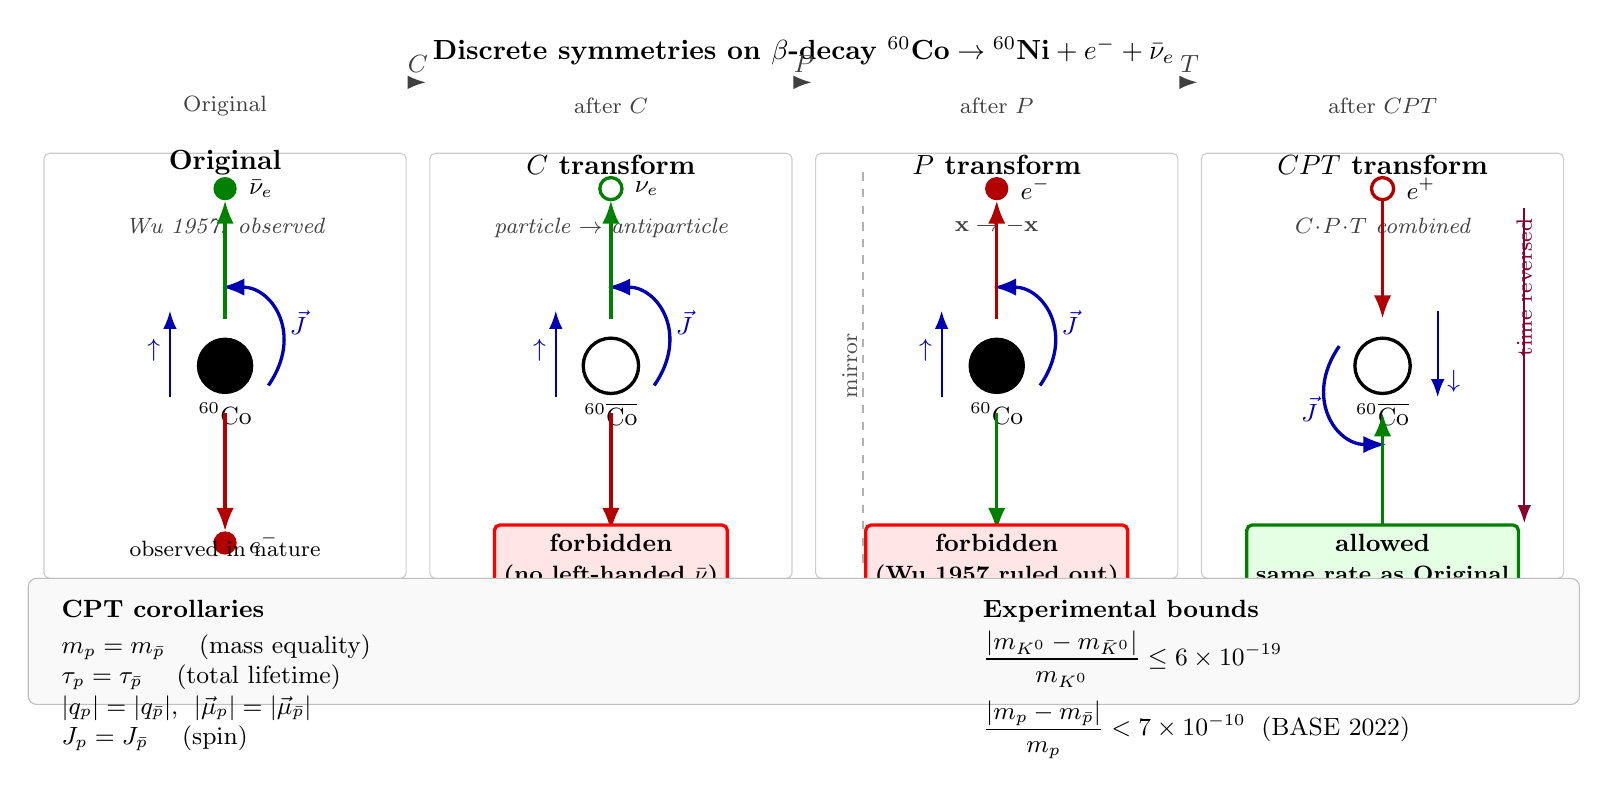
\begin{tikzpicture}[>=Latex, font=\small]

% =====================================================================
% Four panels: Original, C, P, CPT
% Each panel: a beta-decay diagram of 60Co
% =====================================================================

% ---- Geometry constants ----
\def\panelW{4.6}      % panel width
\def\panelH{5.4}      % panel height
\def\gap{0.3}         % gap between panels

% Panel x-centers
\def\xA{0}
\def\xB{\panelW + \gap}
\def\xC{2*\panelW + 2*\gap}
\def\xD{3*\panelW + 3*\gap}

% ============== Panel boundaries (drawn as light frames) ==============
\foreach \xc in {\xA,\xB,\xC,\xD}{
  \draw[gray!40, rounded corners=2pt]
    (\xc-\panelW/2,-\panelH/2) rectangle (\xc+\panelW/2,\panelH/2);
}

% =====================================================================
% Macro to draw a beta-decay event at center (cx,cy)
%
% args:
% #1 = center x
% #2 = center y
% #3 = nucleus label (e.g. {$^{60}\text{Co}$})
% #4 = nucleus fill style (filled / open)
% #5 = spin direction:  up / down
% #6 = electron label  (e^- or e^+)
% #7 = electron filled? (filled / open)
% #8 = electron direction:  down / up   (where it is going)
% #9 = neutrino label  (\bar\nu_e or \nu_e)
% =====================================================================
% Because TikZ allows up to 9 args, the remaining choices are coded
% with separate calls; we will inline each panel for clarity.

% =====================================================================
% Panel A : ORIGINAL PROCESS
%   60Co (filled), spin up, e^- down, anti-nu_e up
% =====================================================================
\begin{scope}[shift={(\xA,0)}]
  % title
  \node[anchor=south, font=\bfseries] at (0,\panelH/2 - 0.4) {Original};
  \node[anchor=north, font=\itshape\footnotesize, gray!50!black]
    at (0,\panelH/2 - 0.7) {Wu 1957: observed};

  % nucleus
  \filldraw[fill=black, draw=black] (0,0) circle (10pt);
  \node[below=10pt] at (0,0) {$^{60}\text{Co}$};

  % spin arrow (curved arrow attached to nucleus, indicating spin up)
  \draw[->, very thick, blue!70!black]
    (0.55,-0.25) .. controls (1.0,0.4) and (0.6,1.0) .. (-0.05,1.0);
  \node[blue!70!black, anchor=west] at (0.7,0.55) {$\vec J$};
  % up-arrow indicator
  \draw[->, thick, blue!70!black] (-0.7,-0.4) -- (-0.7,0.7);
  \node[blue!70!black, anchor=east] at (-0.7,0.2) {$\uparrow$};

  % electron: emitted downward
  \draw[->, very thick, red!70!black] (0,-0.6) -- (0,-2.1);
  \filldraw[fill=red!70!black, draw=red!70!black] (0,-2.25) circle (4pt);
  \node[anchor=west] at (0.18,-2.25) {$e^{-}$};

  % anti-neutrino: emitted upward
  \draw[->, very thick, green!50!black] (0,0.6) -- (0,2.1);
  \filldraw[fill=green!50!black, draw=green!50!black] (0,2.25) circle (4pt);
  \node[anchor=west] at (0.18,2.25) {$\bar{\nu}_{e}$};

  % bottom annotation
  \node[align=center, anchor=north] at (0,-\panelH/2 + 0.6)
    {\footnotesize observed in nature};
\end{scope}

% =====================================================================
% Panel B : C transformation
%   anti-60Co (open), spin up, e^+ down, nu_e up
%   forbidden in nature
% =====================================================================
\begin{scope}[shift={(\xB,0)}]
  \node[anchor=south, font=\bfseries] at (0,\panelH/2 - 0.4) {$C$ transform};
  \node[anchor=north, font=\itshape\footnotesize, gray!50!black]
    at (0,\panelH/2 - 0.7) {particle $\to$ antiparticle};

  % anti-nucleus (open circle)
  \draw[fill=white, draw=black, very thick] (0,0) circle (10pt);
  \node[below=10pt] at (0,0) {$^{60}\overline{\text{Co}}$};

  % spin arrow: SAME direction (J unchanged under C)
  \draw[->, very thick, blue!70!black]
    (0.55,-0.25) .. controls (1.0,0.4) and (0.6,1.0) .. (-0.05,1.0);
  \node[blue!70!black, anchor=west] at (0.7,0.55) {$\vec J$};
  \draw[->, thick, blue!70!black] (-0.7,-0.4) -- (-0.7,0.7);
  \node[blue!70!black, anchor=east] at (-0.7,0.2) {$\uparrow$};

  % positron: still emitted downward (momenta unchanged under C)
  \draw[->, very thick, red!70!black] (0,-0.6) -- (0,-2.1);
  \draw[fill=white, draw=red!70!black, very thick] (0,-2.25) circle (4pt);
  \node[anchor=west] at (0.18,-2.25) {$e^{+}$};

  % neutrino: emitted upward
  \draw[->, very thick, green!50!black] (0,0.6) -- (0,2.1);
  \draw[fill=white, draw=green!50!black, very thick] (0,2.25) circle (4pt);
  \node[anchor=west] at (0.18,2.25) {$\nu_{e}$};

  % "forbidden" stamp
  \node[draw=red, very thick, rounded corners=2pt, fill=red!10,
        font=\bfseries\small, align=center, anchor=north]
    at (0,-\panelH/2 + 0.7)
    {forbidden\\ {\footnotesize (no left-handed $\bar\nu$)}};
\end{scope}

% =====================================================================
% Panel C : P transformation
%   60Co (filled), spin still up (axial vector), momenta REVERSED
%   forbidden (this is what Wu 1957 ruled out)
% =====================================================================
\begin{scope}[shift={(\xC,0)}]
  \node[anchor=south, font=\bfseries] at (0,\panelH/2 - 0.4) {$P$ transform};
  \node[anchor=north, font=\itshape\footnotesize, gray!50!black]
    at (0,\panelH/2 - 0.7) {$\mathbf x \to -\mathbf x$};

  % nucleus (same particle, filled)
  \filldraw[fill=black, draw=black] (0,0) circle (10pt);
  \node[below=10pt] at (0,0) {$^{60}\text{Co}$};

  % mirror line (vertical dashed)
  \draw[gray!60, dashed, thick] (-1.7,-2.5) -- (-1.7,2.5);
  \node[gray!60!black, font=\footnotesize, anchor=south, rotate=90]
    at (-1.65,0) {mirror};

  % spin arrow: STILL up (axial vector, invariant under P)
  \draw[->, very thick, blue!70!black]
    (0.55,-0.25) .. controls (1.0,0.4) and (0.6,1.0) .. (-0.05,1.0);
  \node[blue!70!black, anchor=west] at (0.7,0.55) {$\vec J$};
  \draw[->, thick, blue!70!black] (-0.7,-0.4) -- (-0.7,0.7);
  \node[blue!70!black, anchor=east] at (-0.7,0.2) {$\uparrow$};

  % electron: emitted UPWARD now (momentum reversed by P)
  \draw[->, very thick, red!70!black] (0,0.6) -- (0,2.1);
  \filldraw[fill=red!70!black, draw=red!70!black] (0,2.25) circle (4pt);
  \node[anchor=west] at (0.18,2.25) {$e^{-}$};

  % anti-neutrino: emitted DOWNWARD now (momentum reversed)
  \draw[->, very thick, green!50!black] (0,-0.6) -- (0,-2.1);
  \filldraw[fill=green!50!black, draw=green!50!black] (0,-2.25) circle (4pt);
  \node[anchor=west] at (0.18,-2.25) {$\bar{\nu}_{e}$};

  % "forbidden" stamp
  \node[draw=red, very thick, rounded corners=2pt, fill=red!10,
        font=\bfseries\small, align=center, anchor=north]
    at (0,-\panelH/2 + 0.7)
    {forbidden\\ {\footnotesize (Wu 1957 ruled out)}};
\end{scope}

% =====================================================================
% Panel D : CPT transformation
%   anti-60Co (open), spin DOWN, e^+ up, nu_e down
%   process runs BACKWARDS in time:  e^+ + nu_e -> anti-60Co
%   ALLOWED, with same rate as panel A
% =====================================================================
\begin{scope}[shift={(\xD,0)}]
  \node[anchor=south, font=\bfseries] at (0,\panelH/2 - 0.4) {$CPT$ transform};
  \node[anchor=north, font=\itshape\footnotesize, gray!50!black]
    at (0,\panelH/2 - 0.7) {$C\!\cdot\!P\!\cdot\!T$ combined};

  % anti-nucleus (open)
  \draw[fill=white, draw=black, very thick] (0,0) circle (10pt);
  \node[below=10pt] at (0,0) {$^{60}\overline{\text{Co}}$};

  % spin arrow: DOWN now (T flips J, P keeps it, C keeps it -> net flip)
  \draw[->, very thick, blue!70!black]
    (-0.55,0.25) .. controls (-1.0,-0.4) and (-0.6,-1.0) .. (0.05,-1.0);
  \node[blue!70!black, anchor=east] at (-0.7,-0.55) {$\vec J$};
  \draw[->, thick, blue!70!black] (0.7,0.7) -- (0.7,-0.4);
  \node[blue!70!black, anchor=west] at (0.7,-0.2) {$\downarrow$};

  % time-reversed: incoming particles (arrows pointing INWARD)
  % positron coming from above
  \filldraw[fill=white, draw=red!70!black, very thick] (0,2.25) circle (4pt);
  \draw[->, very thick, red!70!black] (0,2.1) -- (0,0.6);
  \node[anchor=west] at (0.18,2.25) {$e^{+}$};

  % neutrino coming from below
  \filldraw[fill=white, draw=green!50!black, very thick] (0,-2.25) circle (4pt);
  \draw[->, very thick, green!50!black] (0,-2.1) -- (0,-0.6);
  \node[anchor=west] at (0.18,-2.25) {$\nu_{e}$};

  % time-arrow indicator (T reversed)
  \draw[<-, thick, purple!70!black]
    (\panelW/2 - 0.5,-2.0) -- (\panelW/2 - 0.5,2.0);
  \node[purple!70!black, font=\footnotesize, anchor=west, rotate=90]
    at (\panelW/2 - 0.5,0) {time reversed};

  % "allowed" stamp
  \node[draw=green!50!black, very thick, rounded corners=2pt,
        fill=green!10, font=\bfseries\small, align=center, anchor=north]
    at (0,-\panelH/2 + 0.7)
    {allowed\\ {\footnotesize same rate as Original}};
\end{scope}

% =====================================================================
% Bottom info band: CPT corollaries + experimental bounds
% =====================================================================
\def\bandY{-\panelH/2 - 1.6}
\def\bandH{1.6}
\def\bandLeft{-\panelW/2 - 0.2}
\def\bandRight{3*\panelW + 3*\gap + \panelW/2 + 0.2}

\draw[gray!50, rounded corners=3pt, fill=gray!5]
  (\bandLeft,\bandY) rectangle (\bandRight,\bandY+\bandH);

% left half: corollaries
\node[anchor=north west, align=left, font=\small] at (\bandLeft+0.3,\bandY+\bandH-0.15)
  {\textbf{CPT corollaries}\\[2pt]
   $m_{p}=m_{\bar p}$ \quad (mass equality)\\
   $\tau_{p}=\tau_{\bar p}$ \quad (total lifetime)\\
   $|q_{p}|=|q_{\bar p}|,\;\, |\vec\mu_{p}|=|\vec\mu_{\bar p}|$\\
   $J_{p}=J_{\bar p}$ \quad (spin)};

% right half: experimental bounds
\node[anchor=north west, align=left, font=\small] at (\xC - 0.3,\bandY+\bandH-0.15)
  {\textbf{Experimental bounds}\\[2pt]
   $\dfrac{|m_{K^{0}}-m_{\bar K^{0}}|}{m_{K^{0}}} \le 6\times 10^{-19}$\\[4pt]
   $\dfrac{|m_{p}-m_{\bar p}|}{m_{p}} < 7\times 10^{-10}$ \;(BASE 2022)};

% =====================================================================
% Top header: arrow chain showing C, P, T composition
% =====================================================================
\def\headerY{\panelH/2 + 0.9}
\node[anchor=center, font=\bfseries] at (\xA + 1.5*\panelW + 1.5*\gap, \headerY + 0.4)
  {Discrete symmetries on $\beta$-decay $^{60}\text{Co}\to {}^{60}\text{Ni}+e^{-}+\bar\nu_{e}$};

% Chain arrows between panels
\draw[->, thick, gray!50!black] (\xA + \panelW/2 + 0.05, \headerY) -- (\xB - \panelW/2 - 0.05, \headerY)
  node[midway, above, font=\small] {$C$};
\draw[->, thick, gray!50!black] (\xB + \panelW/2 + 0.05, \headerY) -- (\xC - \panelW/2 - 0.05, \headerY)
  node[midway, above, font=\small] {$P$};
\draw[->, thick, gray!50!black] (\xC + \panelW/2 + 0.05, \headerY) -- (\xD - \panelW/2 - 0.05, \headerY)
  node[midway, above, font=\small] {$T$};

% Tiny labels at each panel above the chain
\foreach \xc/\lab in {\xA/{Original},\xB/{after $C$},\xC/{after $P$},\xD/{after $CPT$}}{
  \node[font=\footnotesize, gray!50!black] at (\xc, \headerY - 0.3) {\lab};
}

\end{tikzpicture}
\end{document}
